\chapter{Building a Black Hole and the Near-Horizon Puzzle}

These notes follow Leonard Susskind's fifth supplementary lecture in \emph{Cosmology and Black Holes} and are curated by LazyingArt LLC. The lecture begins with a deliberately rough estimate of a black hole in equilibrium with the \(3\,\mathrm{K}\) microwave background, then turns to a more systematic construction: first rebuild the Penrose-diagram ``working parts'' for flat space and Schwarzschild, then use Birkhoff's theorem to sew together a collapsing shell of light, and finally confront the more delicate question of what one can really mean by temperature and excitation near an event horizon.

\section{Warm-Up: A Three-Degree Black Hole}

Susskind opens with a homework-style estimate: what would the mass of a black hole be if its Hawking temperature were of order the temperature of the cosmic microwave background? The point is not precision. The point is to re-enter the subject through scale.

His lecture heuristic is simple. A black hole of radius \(R_s\) radiates quanta with wavelength of the same order as its own size. At a temperature of a few kelvin, the relevant radiation is in the microwave regime, so he takes the wavelength to be of order centimeters. Thus
\begin{equation}
R_s \sim \lambda_{\text{thermal}} \sim 1\,\mathrm{cm}.
\end{equation}
Now compare this with a solar-mass black hole, whose Schwarzschild radius is of order kilometers. Since the Schwarzschild radius is proportional to the mass,
\begin{equation}
R_s=\frac{2GM}{c^2},
\qquad
\frac{M}{M_\odot}\sim \frac{R_s}{R_{s,\odot}} \sim 10^{-5}.
\end{equation}
This places the mass in the broad range of planetary masses. Susskind estimates roughly an Earth mass; a student reports a value closer to the Moon mass. The lecture treats this only as an order-of-magnitude exercise, and that is the right way to preserve it in the notes.

The physical point is also qualitative. A \(3\,\mathrm{K}\) black hole would be roughly in equilibrium with its surroundings, but not in a stable equilibrium: if it became slightly hotter it would radiate more and heat up further, while if it became slightly colder it would tend to cool further. Having used the estimate to reset the scale, Susskind cuts it off and turns to the real question: how does one \emph{build} a black hole, at least mathematically?

\section{Two Penrose-Diagram Working Parts}

\subsection{Flat Space in Reduced \((t,r)\) Coordinates}

The first working part is the Penrose diagram of flat space, written in terms of time \(t\) and radial distance \(r\). The angular directions are suppressed. Every point of the diagram therefore stands for a two-sphere.

\begin{definition}
In the reduced description used throughout the lecture, the coordinates are \((t,r)\) with \(r\geq 0\), and each point represents a sphere \(S^2\) of angular directions.
\end{definition}

Radial light rays move at \(45^\circ\). Incoming rays run toward \(r=0\); outgoing rays run away from it. The Penrose diagram is obtained by a conformal compactification that brings the infinite half-plane to a finite wedge while preserving the null directions. Susskind jokingly calls this operation ``smushing,'' but the mathematical content is standard: null lines remain null, and the crowding of constant-\(r\) and constant-\(t\) curves near infinity is the geometric signature of the compactification.

\begin{figure}[ht]
\centering

\includegraphics[width=0.62\textwidth]{lecture_05_figure_02.png}
\caption{Susskind's upper-half compactified flat-space Penrose diagram. The lower half is omitted on the board at this stage of the lecture.}
\end{figure}

The screenshot is especially useful because it records exactly what Susskind chose to keep in view: only the upper half, with the left timelike boundary, the top point labeled \(t=\infty\), and the fan of compressed coordinate curves.

\begin{figure}[ht]
\centering
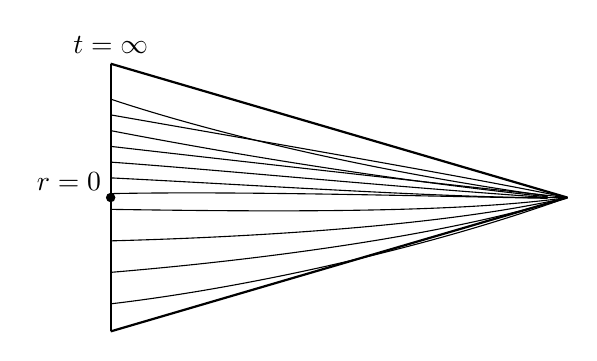
\begin{tikzpicture}[scale=1.0]
\draw[thick] (0,0) -- (0,3.4);
\draw[thick] (0,3.4) -- (5.8,1.7);
\draw[thick] (0,0) -- (5.8,1.7);

\fill (0,1.7) circle (0.06);

\draw (0,0.35) .. controls (1.7,0.55) and (4.0,1.05) .. (5.8,1.7);
\draw (0,0.75) .. controls (1.8,0.90) and (4.2,1.20) .. (5.8,1.7);
\draw (0,1.15) .. controls (1.9,1.20) and (4.3,1.35) .. (5.8,1.7);
\draw (0,1.55) .. controls (2.0,1.52) and (4.4,1.50) .. (5.8,1.7);
\draw (0,1.95) .. controls (2.0,1.85) and (4.5,1.68) .. (5.8,1.7);
\draw (0,2.35) .. controls (2.0,2.12) and (4.6,1.83) .. (5.8,1.7);
\draw (0,2.75) .. controls (2.0,2.40) and (4.6,1.95) .. (5.8,1.7);

\draw (0,2.95) .. controls (1.2,2.55) and (3.2,2.05) .. (5.55,1.72);
\draw (0,2.55) .. controls (1.3,2.30) and (3.3,1.95) .. (5.55,1.71);
\draw (0,2.15) .. controls (1.4,2.05) and (3.4,1.85) .. (5.55,1.70);
\draw (0,1.75) .. controls (1.5,1.78) and (3.5,1.73) .. (5.55,1.69);

\node[left] at (0,1.9) {$r=0$};
\node[above] at (0,3.4) {$t=\infty$};
\end{tikzpicture}
\caption{A cleaned reconstruction of the upper half of the compactified flat-space diagram. The precise curve shapes are qualitative rather than analytic.}
\end{figure}

Two qualitative features matter in the lecture. First, constant-\(r\) worldlines, which are vertical in the unsquashed picture, bunch up as one moves toward infinity. Second, constant-time slices also bunch up toward the top of the diagram. Susskind also remarks that light rays that miss the origin are still nearly indistinguishable from radial rays when far away; only close to the origin do they reveal that they turn around at some minimum radius rather than bounce at \(r=0\).

\subsection{The Schwarzschild Penrose Diagram}

The second working part is the Penrose diagram of the eternal Schwarzschild solution. Susskind redraws it as two adjacent diamonds, with spacelike singularities at the top and bottom. What matters for the lecture is not the full Kruskal extension in all its abstract glory, but the right-hand exterior region, the one that will later be retained in the collapse construction.

\begin{figure}[ht]
\centering

\includegraphics[width=0.72\textwidth]{lecture_05_figure_03.png}
\caption{Susskind's Schwarzschild Penrose diagram, with a hand-drawn family of constant-\(r\) and constant-time curves in the right exterior region.}
\end{figure}

The board labels visible in this frame are enough to anchor the geometry:
\[
t=\infty,\qquad t=-\infty,\qquad r=\infty.
\]
The edge of the exterior region that plays the role of the horizon is the locus
\[
r=2MG,
\]
and Susskind uses representative outer radii such as
\[
r=6MG,\qquad r=100MG
\]
to emphasize that the exterior geometry far from the hole resembles the compactified flat-space picture. That resemblance is the whole point of juxtaposing the two diagrams.

\begin{figure}[ht]
\centering
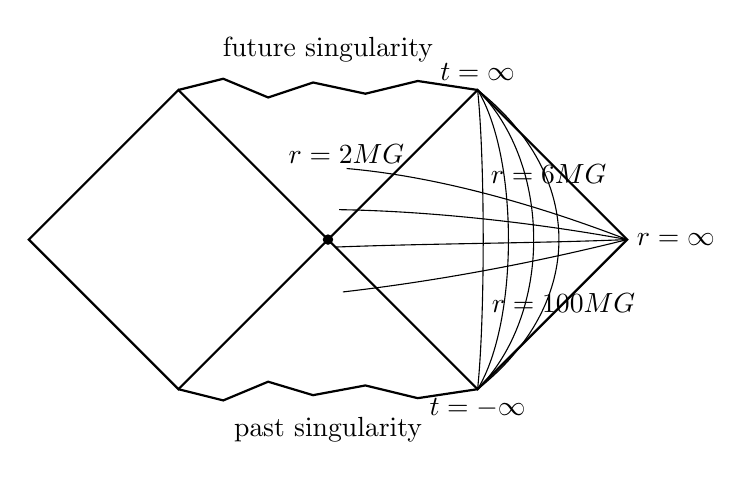
\begin{tikzpicture}[scale=0.95]
\coordinate (C) at (0,0);
\coordinate (LT) at (-2,2);
\coordinate (LL) at (-4,0);
\coordinate (LB) at (-2,-2);
\coordinate (RT) at (2,2);
\coordinate (RR) at (4,0);
\coordinate (RB) at (2,-2);

\draw[thick] (C) -- (LT) -- (LL) -- (LB) -- (C);
\draw[thick] (C) -- (RT) -- (RR) -- (RB) -- (C);

\draw[thick] (-2,2) -- (-1.4,2.15) -- (-0.8,1.9) -- (-0.2,2.1) -- (0.5,1.95) -- (1.2,2.12) -- (2,2);
\draw[thick] (-2,-2) -- (-1.4,-2.15) -- (-0.8,-1.9) -- (-0.2,-2.08) -- (0.5,-1.95) -- (1.2,-2.12) -- (2,-2);

\fill (C) circle (0.07);

\draw (2,2) .. controls (2.10,1.05) and (2.10,-1.05) .. (2,-2);
\draw (2,2) .. controls (2.55,1.10) and (2.55,-1.10) .. (2,-2);
\draw (2,2) .. controls (3.00,1.00) and (3.00,-1.00) .. (2,-2);
\draw (2,2) .. controls (3.45,0.85) and (3.45,-0.85) .. (2,-2);

\draw (0.25,0.95) .. controls (1.4,0.85) and (2.7,0.50) .. (4,0);
\draw (0.15,0.40) .. controls (1.4,0.38) and (2.8,0.22) .. (4,0);
\draw (0.10,-0.10) .. controls (1.4,-0.05) and (2.8,-0.05) .. (4,0);
\draw (0.20,-0.70) .. controls (1.5,-0.55) and (2.8,-0.30) .. (4,0);

\node[above] at (2,2) {$t=\infty$};
\node[below] at (2,-2) {$t=-\infty$};
\node[right] at (4,0) {$r=\infty$};
\node[left] at (1.15,1.15) {$r=2MG$};
\node at (2.95,0.88) {$r=6MG$};
\node at (3.15,-0.85) {$r=100MG$};
\node[above] at (0.0,2.25) {future singularity};
\node[below] at (0.0,-2.25) {past singularity};
\end{tikzpicture}
\caption{A cleaned reconstruction of the Schwarzschild diagram used in the lecture. The internal grid is schematic: it records the intended coordinate reading rather than an exact plot.}
\end{figure}

The comparison with flat space is essential. In the reduced flat diagram, light rays can reach \(r=0\) and bounce. In Schwarzschild, once a light ray has crossed the horizon it does not bounce from a center. It continues to the singularity. This is why the two compactified pictures look similar in the asymptotic region and profoundly different near the hole.

\section{Newton's Shell Theorem and Birkhoff's Theorem}

At this point Susskind inserts the theorem that makes the dynamical construction possible. He first recalls Newton's shell theorem, then immediately upgrades it to the relativistic statement he needs.

\begin{theorem}[Newton shell theorem, in the form used here]
For a spherically symmetric distribution of mass, the gravitational field at radius \(r\) depends only on the mass contained inside the sphere of radius \(r\). In particular, inside a hollow spherical shell the gravitational field vanishes, while outside the shell the field is the same as if the entire mass were concentrated at the center.
\end{theorem}

For the special case of a thin spherical shell of total mass \(M\), one may summarize the Newtonian result as
\begin{equation}
g_{\text{inside shell}}=0,
\qquad
g_{\text{outside shell}}=\frac{GM}{r^2}.
\end{equation}
Susskind does not pause on the formula. What he wants is the logical structure: the inside and outside are governed by different but very simple rules.

\begin{theorem}[Birkhoff's theorem, in the operational form of the lecture]
Inside a spherically symmetric shell, spacetime is flat Minkowski spacetime. Outside the shell, spacetime is Schwarzschild with the shell's total mass.
\end{theorem}

The lecture stresses two points. First, this need not be a static shell. As long as spherical symmetry is preserved, the theorem still applies in the simple form Susskind needs. Second, the theorem applies not only to material shells but equally to a shell of radiation. This is the bridge from the familiar static Schwarzschild geometry to a genuine process of formation.

\section{A Black Hole from a Collapsing Shell of Light}

Susskind's simplest black-hole formation model is an ingoing spherical shell of light. If the shell carries total energy \(E\), then as measured from far away it carries the mass parameter
\begin{equation}
M=\frac{E}{c^2}.
\end{equation}
In the lecture he immediately suppresses the distinction by working in natural units and speaking informally of the shell as a ``mass \(M\)'' moving at the speed of light.

The strategic use of Birkhoff's theorem is now transparent. At any given moment,
\begin{itemize}
\item inside the shell the geometry is flat spacetime,
\item outside the shell the geometry is Schwarzschild.
\end{itemize}
The shell itself is the seam where the two regions are sewn together.

\begin{figure}[ht]
\centering

\includegraphics[width=0.72\textwidth]{lecture_05_figure_05.png}
\caption{Board layout at the moment Susskind turns from the two Penrose-diagram working parts to the collapsing-shell construction.}
\end{figure}

The transition frame is important precisely because it is not yet the final collapse diagram. One still sees the flat-space wedge on the left and the Schwarzschild diagram on the right. The lecture is announcing, almost literally, that these are about to be pasted together.

The construction can be written as an explicit sequence.

\begin{enumerate}
\item Begin with the Penrose diagram of empty flat space.
\item Draw an ingoing null line representing a shell of light arriving from infinity.
\item Use Birkhoff's theorem to keep the region \emph{inside} the shell flat.
\item Use Birkhoff's theorem to replace the region \emph{outside} the shell by the exterior part of the Schwarzschild geometry.
\item Discard the unphysical white-hole region and the second asymptotic exterior of the eternal Schwarzschild diagram.
\item Match the endpoint where the shell reaches the center with the \(r=0\) singular endpoint of the exterior black-hole geometry.
\end{enumerate}

\begin{figure}[ht]
\centering
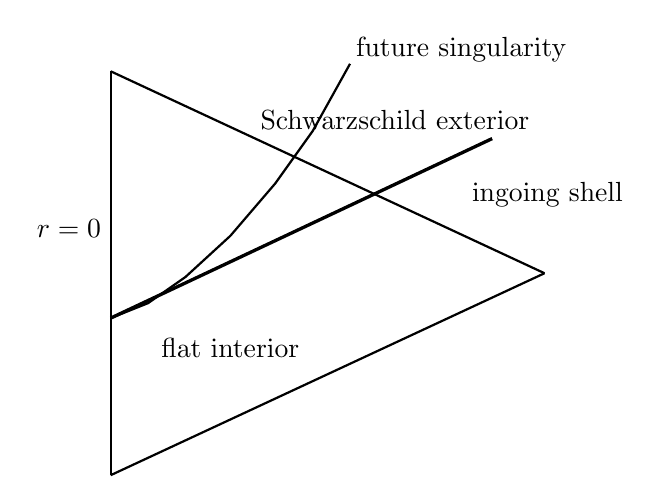
\begin{tikzpicture}[scale=0.95]
\coordinate (O) at (0,-2.3);
\coordinate (P) at (0,3.1);
\coordinate (I) at (5.8,0.4);
\coordinate (S0) at (5.1,2.2);
\coordinate (C0) at (0,-0.2);
\coordinate (T1) at (3.2,3.2);

\draw[thick] (O) -- (P);
\draw[thick] (P) -- (I);
\draw[thick] (O) -- (I);

\draw[very thick] (S0) -- (C0);

\draw[thick] (0,-0.2) -- (0.5,0.0) -- (1.0,0.35) -- (1.6,0.9) -- (2.2,1.6) -- (2.7,2.3) -- (3.2,3.2);

\node[left] at (0,1.0) {$r=0$};
\node[right] at (4.7,1.45) {ingoing shell};
\node at (1.6,-0.6) {flat interior};
\node at (3.8,2.45) {Schwarzschild exterior};
\node[above right] at (3.15,3.1) {future singularity};
\end{tikzpicture}
\caption{A schematic collapse diagram: below the ingoing shell the spacetime is flat, while above it the exterior geometry is Schwarzschild. The shape is qualitative but the causal organization is the one used in the lecture.}
\end{figure}

Susskind emphasizes that this is already enough to explain why the eternal Kruskal picture contains too much. The white hole is gone. The second exterior universe is gone. What remains is the portion of Schwarzschild spacetime that is actually produced by the collapsing shell.

\section{The True Event Horizon}

Once the collapse geometry has been assembled, Susskind asks the next question immediately: where is the horizon? His answer is not to reuse the static label \(r=2MG\) as a definition. The real definition is causal.

\begin{definition}
The event horizon is the boundary in spacetime separating events from which an outgoing light ray can still reach infinity from events from which no outgoing light ray can escape to infinity.
\end{definition}

This definition produces the most striking feature of the lecture. In the collapse diagram the horizon is obtained by tracing the outgoing null line that \emph{just fails} to escape. When this is done, the horizon extends backward into a region that is still locally flat and in which the shell has not yet arrived.

\begin{figure}[ht]
\centering
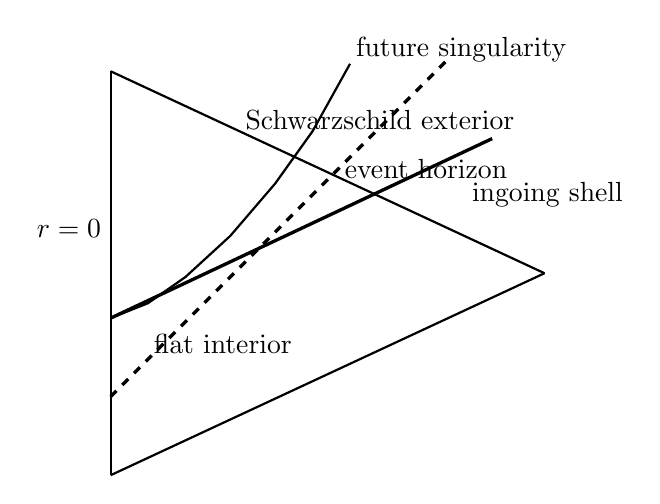
\begin{tikzpicture}[scale=0.95]
\coordinate (O) at (0,-2.3);
\coordinate (P) at (0,3.1);
\coordinate (I) at (5.8,0.4);
\coordinate (S0) at (5.1,2.2);
\coordinate (C0) at (0,-0.2);
\coordinate (H0) at (0,-1.25);

\draw[thick] (O) -- (P);
\draw[thick] (P) -- (I);
\draw[thick] (O) -- (I);

\draw[very thick] (S0) -- (C0);

\draw[thick] (0,-0.2) -- (0.5,0.0) -- (1.0,0.35) -- (1.6,0.9) -- (2.2,1.6) -- (2.7,2.3) -- (3.2,3.2);

\draw[dashed,very thick] (H0) -- (2.6,1.35) -- (4.5,3.25);

\node[left] at (0,1.0) {$r=0$};
\node[right] at (4.7,1.45) {ingoing shell};
\node[right] at (3.0,1.8) {event horizon};
\node at (1.5,-0.55) {flat interior};
\node at (3.6,2.45) {Schwarzschild exterior};
\node[above right] at (3.15,3.1) {future singularity};
\end{tikzpicture}
\caption{The causal horizon in the collapse geometry. The dashed line is the event horizon: it begins in the flat interior before the shell arrives and later becomes the usual Schwarzschild horizon.}
\end{figure}

This is the payoff of the section. A point may lie in flat spacetime and nevertheless already be doomed: no signal sent from that point can ever reach infinity, because the future collapse has already fixed the global causal structure. Susskind makes this intuitive with the drain-hole analogy. One can be sitting in perfectly calm water and yet already be past the point from which escape will remain possible after the plug is pulled.

The horizon is also a growing sphere. Since every point in the reduced diagram stands for a two-sphere, the horizon begins at zero size, grows along the null boundary, and eventually reaches the static Schwarzschild value. In the lecture's shorthand,
\begin{equation}
R_H:\ 0 \longrightarrow 2MG.
\end{equation}
After that it remains fixed unless more matter or radiation is thrown in.

\begin{remark}
The observer-dependent discussion that follows in the lecture belongs here. A distant observer can see the shell come in and can therefore know that a black hole forms, yet the same observer describes infalling matter as piling up near the horizon. Susskind does not resolve that tension here; he uses it to prepare the later discussion of entropy, temperature, and information.
\end{remark}

\section{Hawking Temperature and the Near-Horizon Atmosphere}

Having built the black hole and located the horizon, Susskind shifts from causal geometry to thermodynamics. He begins with the established facts from earlier lectures: black holes have entropy, the entropy is proportional to the horizon area, and adding information to the hole increases the horizon area by Planckian amounts. He then recalls the Hawking temperature.

In the lecture's natural-units convention the formula is quoted as
\begin{equation}
T_H=\frac{\hbar c^3}{8\pi G M},
\end{equation}
while the canonical SI form is
\begin{equation}
T_H=\frac{\hbar c^3}{8\pi G M k_B}.
\end{equation}
Using
\begin{equation}
R_s=\frac{2GM}{c^2},
\end{equation}
one finds
\begin{equation}
T_H=\frac{\hbar c}{4\pi k_B R_s},
\end{equation}
and therefore, in particular,
\begin{equation}
T_H\propto \frac{1}{R_s}.
\end{equation}
This is the relation Susskind wants: large black holes are cold.

The lecture then slows down deliberately. What does temperature mean in a gravitational field? Susskind's answer is operational rather than axiomatic. A thermometer measures the kinetic energy of the particles or photons that hit it. In a gravitational field, those particles lose energy when they climb and gain energy when they fall, so two thermometers placed at different heights need not record the same reading even in a state that is in an appropriate global equilibrium. He illustrates this first with molecules above the Earth's surface, then with photons.

This is the cue for the near-horizon extrapolation. The Hawking temperature \(T_H\) is the temperature measured far from the black hole. If one extrapolates inward, the local temperature rises. Very near the horizon, with \(\rho\) the proper distance from the horizon, Susskind states the result
\begin{equation}
T(\rho)=\frac{1}{2\pi \rho},
\end{equation}
in natural units \(c=\hbar=k_B=1\). The important point is not the derivation, which he postpones, but the qualitative behavior:
\[
\rho\to 0 \qquad \Longrightarrow \qquad T(\rho)\to \infty.
\]
This suggests a very hot near-horizon atmosphere for static probes. A thermometer lowered on a cable will register higher and higher temperatures as it approaches the horizon. Susskind treats that as a legitimate calculation, and in the lecture he insists that it is not a result to be dismissed.

\section{The Operational Puzzle and the Heisenberg Argument}

At this stage the lecture arrives at its sharpest tension. On the one hand, the local temperature near the horizon becomes arbitrarily large for a thermometer held at fixed \(\rho\). On the other hand, a freely falling observer crossing the horizon is not supposed to encounter anything locally dramatic in a large black hole; the geometry near the horizon is still nearly flat.

Susskind formulates the puzzle with an atom. If the atom enters a region where the local temperature exceeds the ionization threshold, then from one point of view it ought to be ionized before crossing the horizon. But from the freely falling point of view one wants to say that nothing particularly special happens at the crossing itself. The lecture does not settle this by declaring one viewpoint correct and the other mistaken. Instead, it asks what experiment could decide the issue.

Before applying that logic to the black hole, Susskind briefly restates the Heisenberg argument. To resolve a particle within a distance \(\Delta x\), one must use light with wavelength no larger than \(\Delta x\):
\begin{equation}
\lambda \lesssim \Delta x.
\end{equation}
Hence the probe photon must carry momentum of order
\begin{equation}
p_\gamma \gtrsim \frac{\hbar}{\Delta x}.
\end{equation}
That is enough to recoil the particle and spoil any attempt to verify simultaneously that it was sharply localized and at rest. The measurement creates the condition it was meant to deny.

The near-horizon experiment follows the same pattern. Let \(\rho\) be the proper distance from the horizon at which the local temperature reaches the ionization scale of the atom. Once the atom enters that layer, the remaining proper time before it crosses the horizon is of order
\begin{equation}
\Delta t \sim \frac{\rho}{c}.
\end{equation}
To determine whether the atom is still intact during that short interval, the outside observer must resolve it over a distance of order \(\rho\). That requires
\begin{equation}
\lambda \lesssim \rho,
\end{equation}
and therefore a probe energy
\begin{equation}
E_\gamma \sim p_\gamma c \gtrsim \frac{\hbar c}{\rho}.
\end{equation}
But this is precisely the same parametric scale as the local thermal energy,
\begin{equation}
E_\gamma \sim \frac{1}{\rho} \sim T(\rho)
\qquad
(c=\hbar=k_B=1).
\end{equation}
So the measurement does not passively reveal whether the atom was ionized by the near-horizon atmosphere. The measurement itself supplies enough energy to ionize or destroy the atom. This is the catch-22 at the end of the lecture.

\begin{remark}
Susskind phrases the conclusion carefully. The argument is not that one has proved, once and for all, what an unmeasured freely falling atom \emph{really} experiences. The conclusion is weaker and operational: no external experiment can confirm the statement ``nothing happened'' without introducing quanta energetic enough to invalidate the very claim being tested.
\end{remark}

He extends the same point to thermometers, laboratories falling with the atom, and signals emitted from the near-horizon region. Any information that reaches the outside must be carried by quanta, and the energy budget required to extract that information is of the same order as the thermal scale near the horizon. Thus the lecture closes not with a metaphysical resolution, but with a sharply framed experimental limitation.

\section{Summary}

The lecture proceeds in a tightly controlled order. A rough \(3\,\mathrm{K}\) estimate sets the scale. Flat-space and Schwarzschild Penrose diagrams are rebuilt as working parts. Newton's theorem and Birkhoff's theorem then permit a genuine collapse construction from an ingoing shell of light. That construction reveals the event horizon as a causal boundary rather than merely the static surface \(r=2MG\), and it exposes the curious fact that the horizon reaches into regions that are still locally flat.

Only after that causal picture is in place does Susskind return to entropy and Hawking temperature. The asymptotic temperature \(T_H\) is small for large holes, but the local extrapolated temperature \(T(\rho)=1/(2\pi\rho)\) becomes large near the horizon. The final Heisenberg-style argument shows why that near-horizon temperature cannot be operationally disentangled from the violent influence of the very measurements designed to test it. In that sense, the lecture ends exactly where it wants to end: with a sharpened puzzle and a precise statement of what physics can, and cannot, presently ask.